\documentclass[11pt]{article}
\usepackage[utf8]{inputenc}
\usepackage{amsmath}
\usepackage{graphicx}
%Gummi|065|=)
\title{\textbf{Trabajo Practico\\
Laboratorio de Redes y Sistemas Operativos}}
\author{Britez Fabrizio\\Daprá Sebastian\\Frischetti Julian}
\date{Diciembre 2016}


\begin{document}

\maketitle

\tableofcontents{}


\clearpage

\section{Definición y alcance}
A lo largo de este proyecto se trabajará para dar explicación detallada de como realizar la instalación y puesta en marcha de un servidor de gestor de archivos. El software elegido es NextCloud.
Tambien se intenrará desarrollar un isntalador, que automatice esta explicación detallada para poder ser ejecutado en cualquier sistema operativo basado en Unix.

\section{NextCloud ¿Qué es?.}

NextCloud es una aplicación de software libre que te permitirá crear un servidor de archivos en la nube, en el cuál podrás tener un almacén de imágenes, documentos o incluso tu música, datos a los que tendrás acceso desde cualquier lugar con internet.

Esta aplicación es un fork de OwnCloud, creada por el mismo creador de Owncloud pero con una tendencia mas abierta y poniendo más enfasis e importancia a la comunidad de simpatizantes y desarrolladores que detrás del proyecto lo hagan crecer. 
\begin{figure}[htp]
\centering
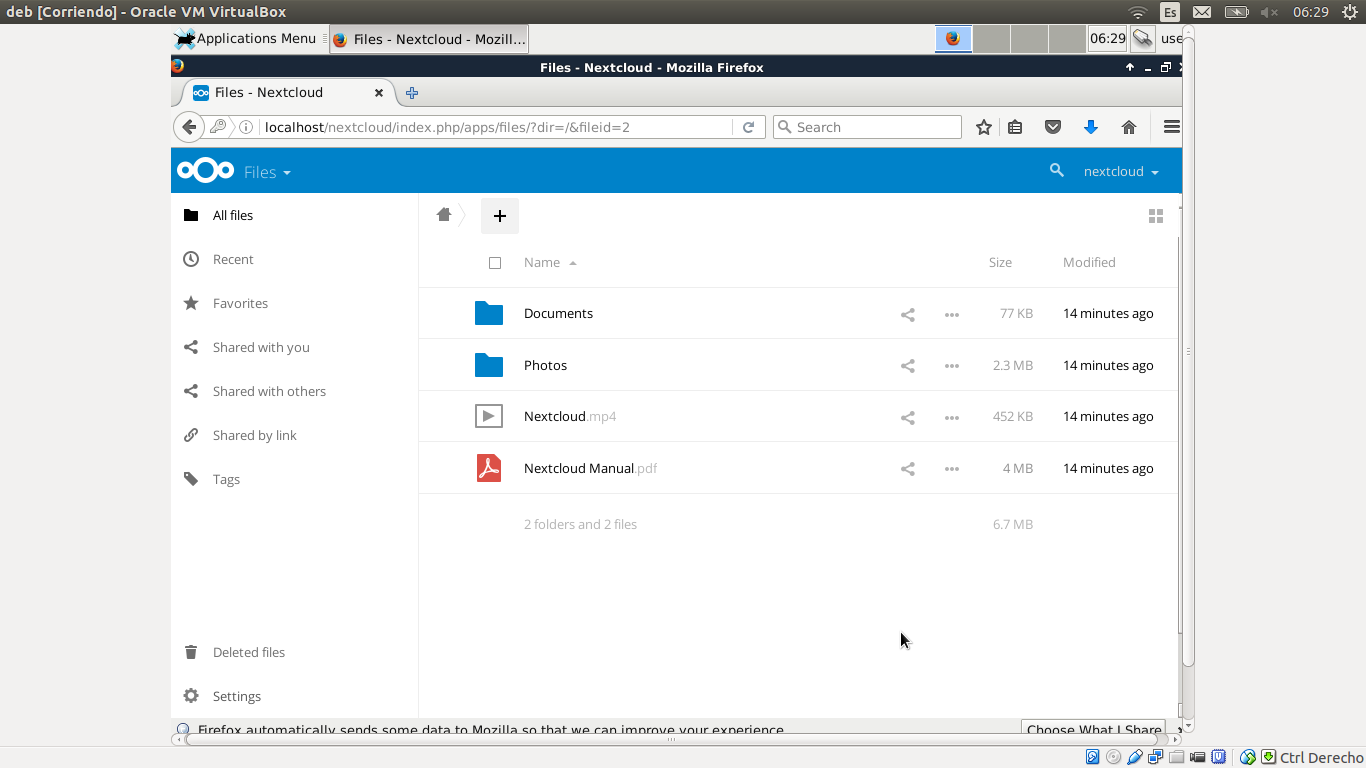
\includegraphics[scale=0.30]{nexcloud2.png}
\caption{Pantalla inicial}
\label{}
\end{figure}

\clearpage

\section{Instalacion Manual en Linux}

Para instalar de forma manual en un sistema operativo basado en Unix se deben seguir los siguientes pasos:

\subsection{Pre requsítos}

Previamente a poner operativo el programa, se deberan instalar algunos programas y librerias para que NextCloud funcione correctamente.
Las mismas son:
\begin{itemize}
    \item Lenguaje y librerias PHP.
    \item Apache2.
    \item Motor de base de datos SQL: MariaDB .
\end{itemize}

Para ello se deben ejecutar desde la terminal los siguientes comandos:

\begin{quote}
\emph{sudo apt-get install apache2}\\
\emph{sudo apt-get install mariadb-server}\\
\emph{sudo apt-get install php5}\\
\emph{sudo apt-get install libapache2-mod-php5}\\
\emph{sudo apt-get install php5-gd}\\
\emph{sudo apt-get install php5-json}\\
\emph{sudo apt-get install php5-mysql}\\
\emph{sudo apt-get install php5-curl}\\
\emph{sudo apt-get install php5-intl}\\
\emph{sudo apt-get install php5-mcrypt}\\
\emph{sudo apt-get install php5-imagick}\\
\end{quote}


\subsection{Obtener NextCloud}
Para obtener una version del servidor de NextCloud podemos descargar un archivo comprimido .zip o .tar.gz de la pagina oficial de NextCloud \emph{www.nextcloud.com/install}.

\begin{figure}[htp]
\centering
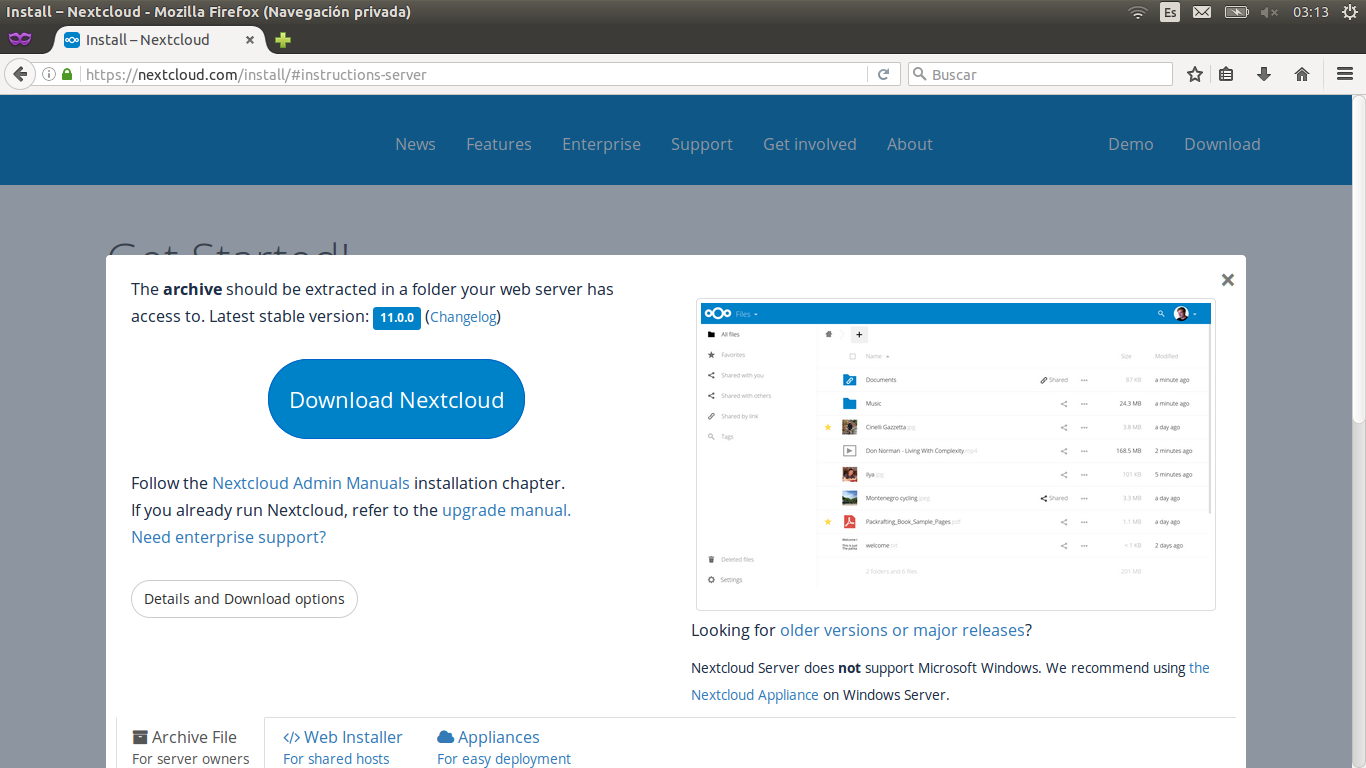
\includegraphics[scale=0.30]{download2.png}
\caption{Descarga web del archivo comprimido}
\label{}
\end{figure}
O bien ejecutando la siguiente linea de consola:
\begin{quote}
\emph{sudo wget https://download.nextcloud.com/server/releases/nextcloud-version.zip}\\
\end{quote}

Donde version, deber reemplazarse por la version actualizada. Al la fecha la version actualizada es nextcloud-11.0.0

\subsection{Ubicar NextCloud en nuestro sistema}
Tenemos el archivo comprimido que contiene todo lo necesario para ejecutar NextCloud, pero necesitamos ponerlo operativo en un servidor (para esto hemos instalado apache2). Entonces descomprimimos el archivo en el directorio de nuestro servidor utilizando el siguiente comando por consola:

\begin{quote}
\textbf{En caso de un tar.bz:}\\
\emph{tar -xjf nextcloud-x.y.z.tar.bz2 -d /var/www}\\\\
\textbf{En caso de un .zip:}\\
\emph{unzip nextcloud-x.y.z.zip -d /var/www}
\end{quote}
	
\subsection{Configuración de bases de datos y servidor}
Antes de proceder a la ejecucion de NextCloud, debemos configurar la base de datos que utilizaremos como asi tambien el servidor donde pondremos operativo el programa.

\subsubsection{Configuración servidor (Apache2)}
Luego de haber instalado Apache2 y darle permismos de lectura y escritura a los archivos  \emph{/var/www/nextcloud/} y \emph{/etc/apache2/sites-enabled} debemos configrar el alias de NextCloud.

\begin{quote}
\emph{
echo "Alias /nextcloud "/var/www/nextcloud/"}\\
\emph{$<$Directory /var/www/nextcloud/$>$}\\
\emph{Options +FollowSymlinks}\\
\emph{AllowOverride All}\\
\emph{ $<IfModule mod_dav.c>$}\\
\emph{Dav off}\\
\emph{$<$/IfModule$>$}\\
\emph{SetEnv HOME /var/www/nextcloud}\\
\emph{$SetEnv HTTP_HOME /var/www/nextcloud$}\\
\emph{$<$/Directory$>$" $>$ /etc/apache2/sites-available/nextcloud.conf}
\end{quote} 

Posteriomente, establecemos un enlace simbolico con el siguiente comando:

\begin{quote}
\emph{ 
ln -s /etc/apache2/sites-available/nextcloud.conf /etc/apache2/sites-enabled/nextcloud.conf
}
\end{quote}

\subsubsection{Configuracion de la base de datos(MariaDB)}

Nuestro motor de base de datos SQL elegido es MariaDB. LA unica configuracion necearia para poder poner en marcha NextCloud, es crear la base de datos donde se persistira la informacion. Podemos hacer todo esto, con la siguiente linea de comando:

\begin{quote}
\emph{ 
mysql -u usuario -pcontrasenia -e "CREATE DATABASE IF NOT EXISTS nextcloud" 
}
\end{quote}

Donde \textbf{usuario} y \textbf{contrasenia} deben ser el usuario y contraseña de administrador de la base de datos que acabamos de crear.

\subsection{Poner a andar NextCloud}
Para poner a andar NexCloud, otorgar los siguientes permisos en la carpeta del servidor:

\begin{quote}
\emph{ 
sudo chown -R www-data:www-data /var/www/nextcloud/ 
}
\end{quote}

Luego, debemos posicionarnos en la carpeta de nuestro servidor donde descomprimimos NextCloud

\begin{quote}
\emph{cd /var/www/nextcloud/}
\end{quote}

y ejecutar utilizando el programa \emph{occ} de php proceder a la instalacion del servidor de NextCloud 

\begin{quote}
\emph{sudo -u www-data php occ  maintenance:install --database "mysql" --database-name "nextcloud"  --database-user "usuario" --database-pass contrasenia --admin-user "usuario adminitrador" --admin-pass "contraseñia administrador"}
\end{quote}

Donde \textbf{usuario} y \textbf{contrasenia} son el usuario y contrasnia de la base de datos que creamos anteriormente y \textbf{usuario administrador} y \textbf{contrasenia administrador}, son el usuario y la contraseña que van a tener el usuario administrador de NextCloud.\\

Una vez finalizada la instalacion, que nos mostrara la siguiente consola:\\
\begin{figure}[htp]
\centering
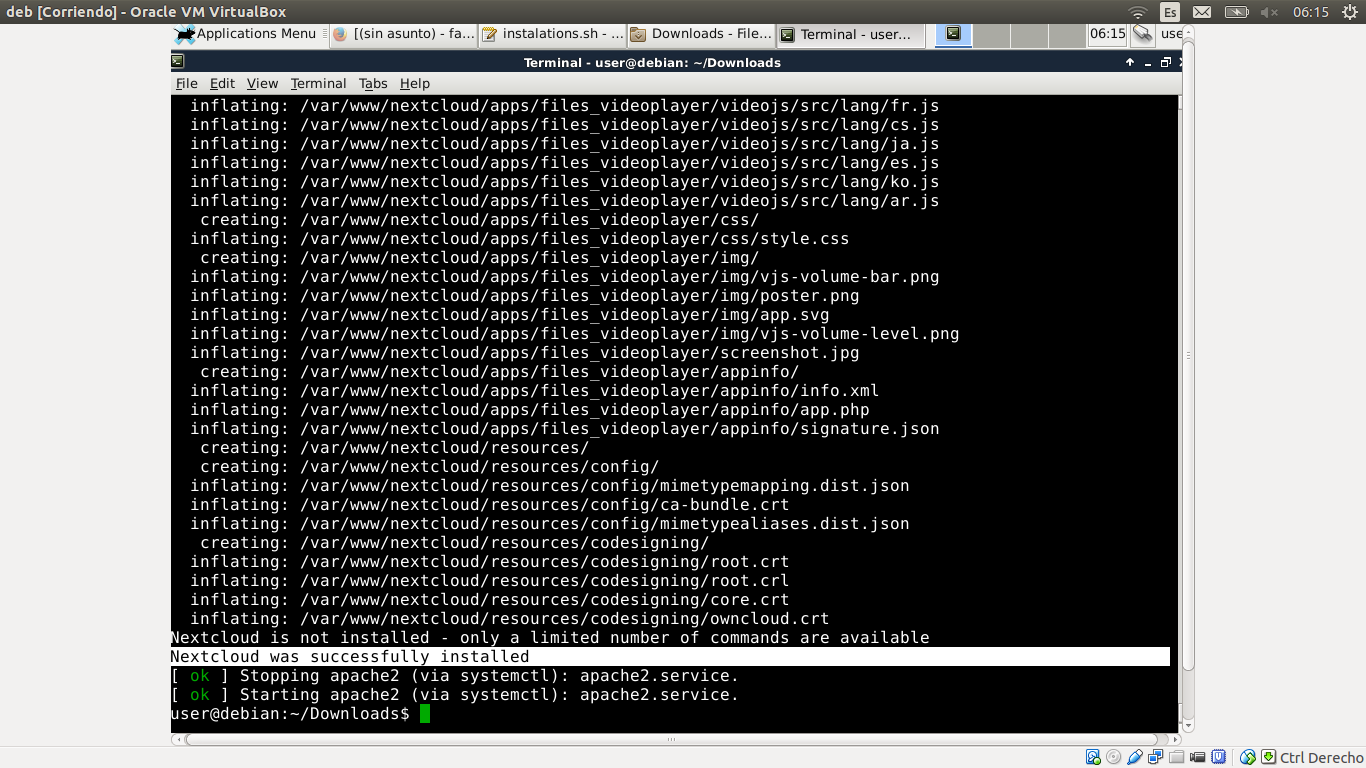
\includegraphics[scale=0.20]{isntalacionCorrecta.png}
\caption{Instalacion correcta}
\label{}
\end{figure}\\

Solo queda reiniciar nuestro servidor con los siguientes comandos:
\begin{quote}
\emph{sudo /etc/init.d/apache2 stop\\
sudo /etc/init.d/apache2 start}
\end{quote}

Y accediendo desde un navegador a \emph{localhost/nextcloud} y se vera:
\begin{figure}[htp]
\centering
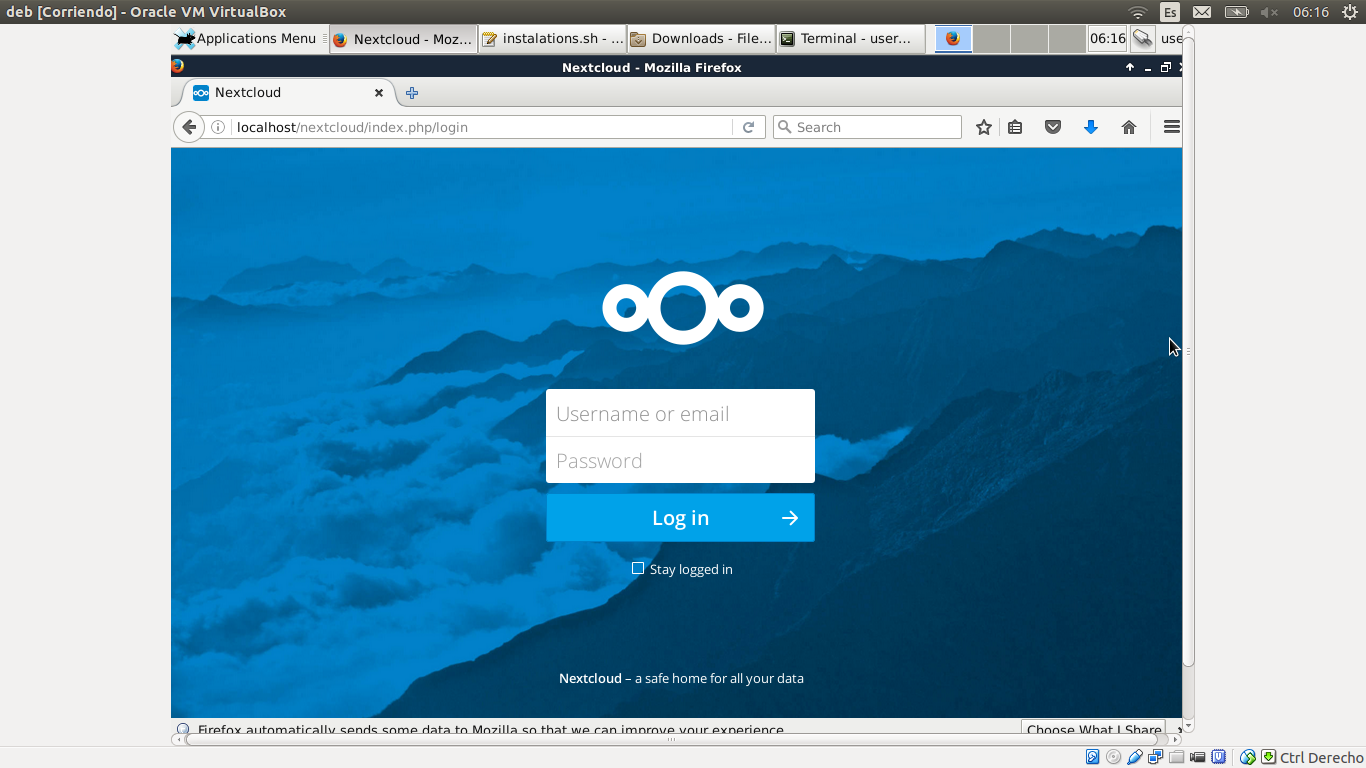
\includegraphics[scale=0.30]{nextcloud1.png}
\caption{Vista de la ventana inicial de NextCloud}
\label{}
\end{figure}

\clearpage


\section{Instalador Automatico en Linux}
Este es el instructivo para usar el instalador automatico de NextCloud.
Este instalador puede usarse tanto en un sistema con interfaz grafica como sin interfaz grafica.
Para lanzar el instalador sin interface grafica se debe ejecutar:

\begin{quote}
\emph{/ubicacionArchivo/sudo sh instalador.sh nonInteractive /rutaDelArchivoComprimidoDeNextCloud/nextcloud-version usuario contrasenia}
\end{quote}

Donde \textbf{nonInteractive} es una palabra que le indica al script que no tiene que levantar interfaz grafica y que correr la instalación directamente informando lo necesario por consola. \textbf{/rutaDelArchivoComprimidoDeNextCloud/} es la ruta donde esta el archivo comprimido del servidor de NexCloud. \textbf{usuario} y \textbf{contrasenia} son los usuario y contraseña de la base de datos que en caso de no tener motor de base de datos instalado, esos valores seran los que quedaran en la configuracion.

Para lanzar el instalador automatico se debe ejecutar la misma linea anterior pero sin parametros la terminal:\\
\begin{quote}
\emph{/ubicacionArchivo/sudo sh instalador.sh}
\end{quote}

Mensaje de Bienvenida. Ademas solicita las contraseñas de la base de datos.\\\\
\begin{figure}[htp]
\centering
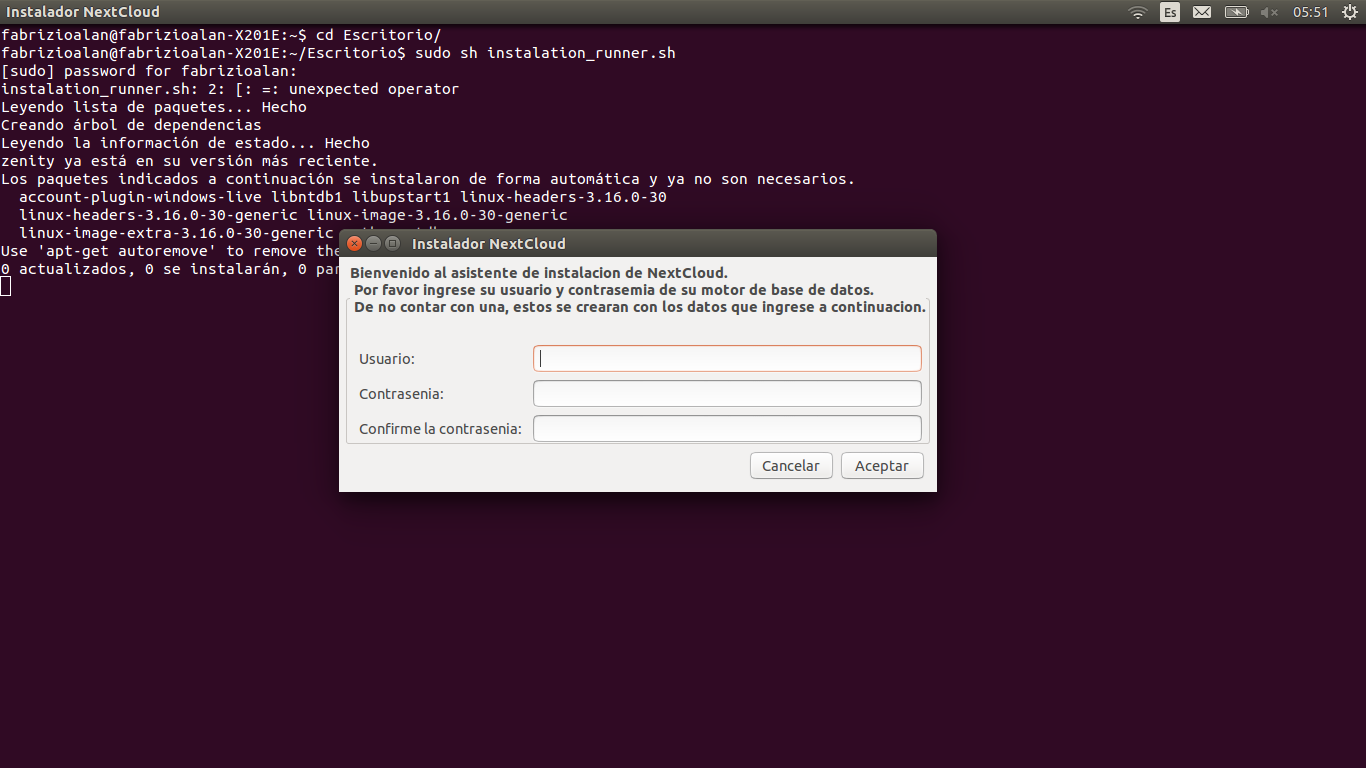
\includegraphics[scale=0.30]{instalador.png}
\caption{}
\label{}
\end{figure}

Seleccion de los archivos comprimidos para llevar acabo la instalacion:

\begin{figure}[htp]
\centering
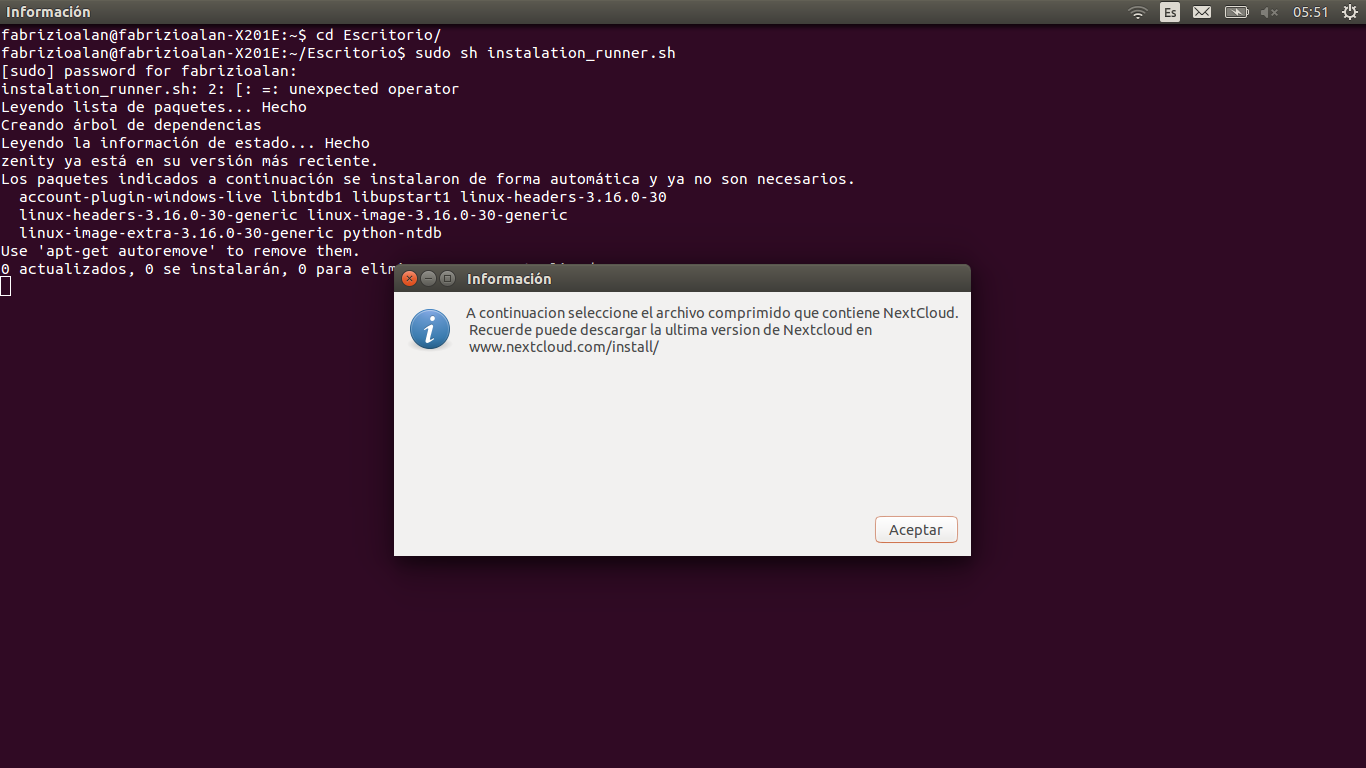
\includegraphics[scale=0.30]{selec.png}
\caption{}
\end{figure}
\begin{figure}[htp]
\centering
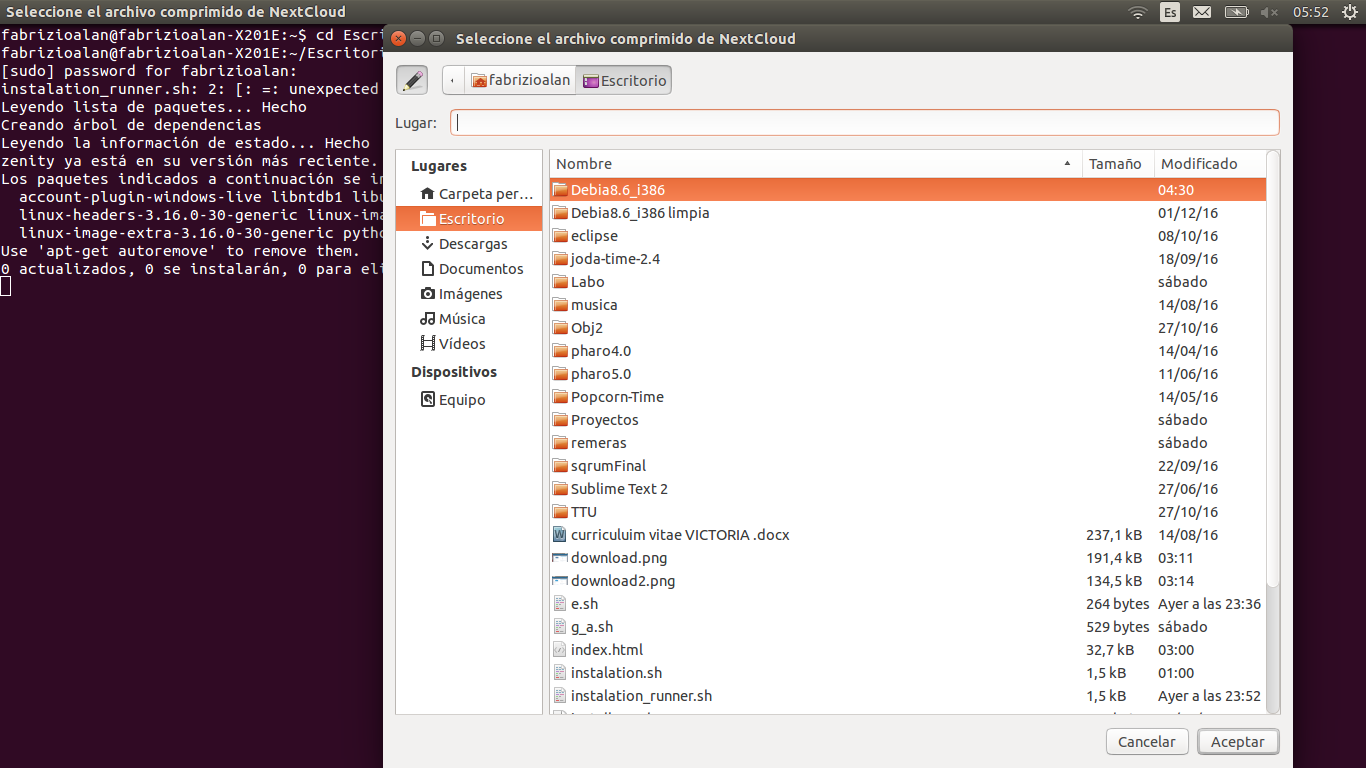
\includegraphics[scale=0.30]{selec2.png}
\end{figure}

\section{Detalles extras del trabajo}

\subsection{Ambiente de pruebas}
Todos los procesos y scripts fueron probados en una maquina virtual con Debian Jesee instalado para probar el los script funcionando en sistemas operativos con lo minimo e indispensable.

\subsection{Dificultades}
Una de las mayores dificultades fue lograr la correcta configuracion de los script bash para que tengan interaccion casi nula con el usuario, para lograr la mayor automatización de la isntalacion. 


\end{document}